%% \chapter[htoc-titlei][hhead-titlei]{htitlei}
%% -----------------------------------------------------------------------------
\chapter[The LHC and the ATLAS experiment][The LHC and ATLAS]
        {The LHC and the ATLAS experiment}
\label{ch:lhc}

%% ------------------------------------------------------------------------------
\FloatBarrier
\section{The LHC}

{\color{red}Standard boring stuff about the LHC accelerator complex, and there
  are four major experiments, blah blah blah. This shouldn't be too long}

\begin{figure}[ht]
  \centering
  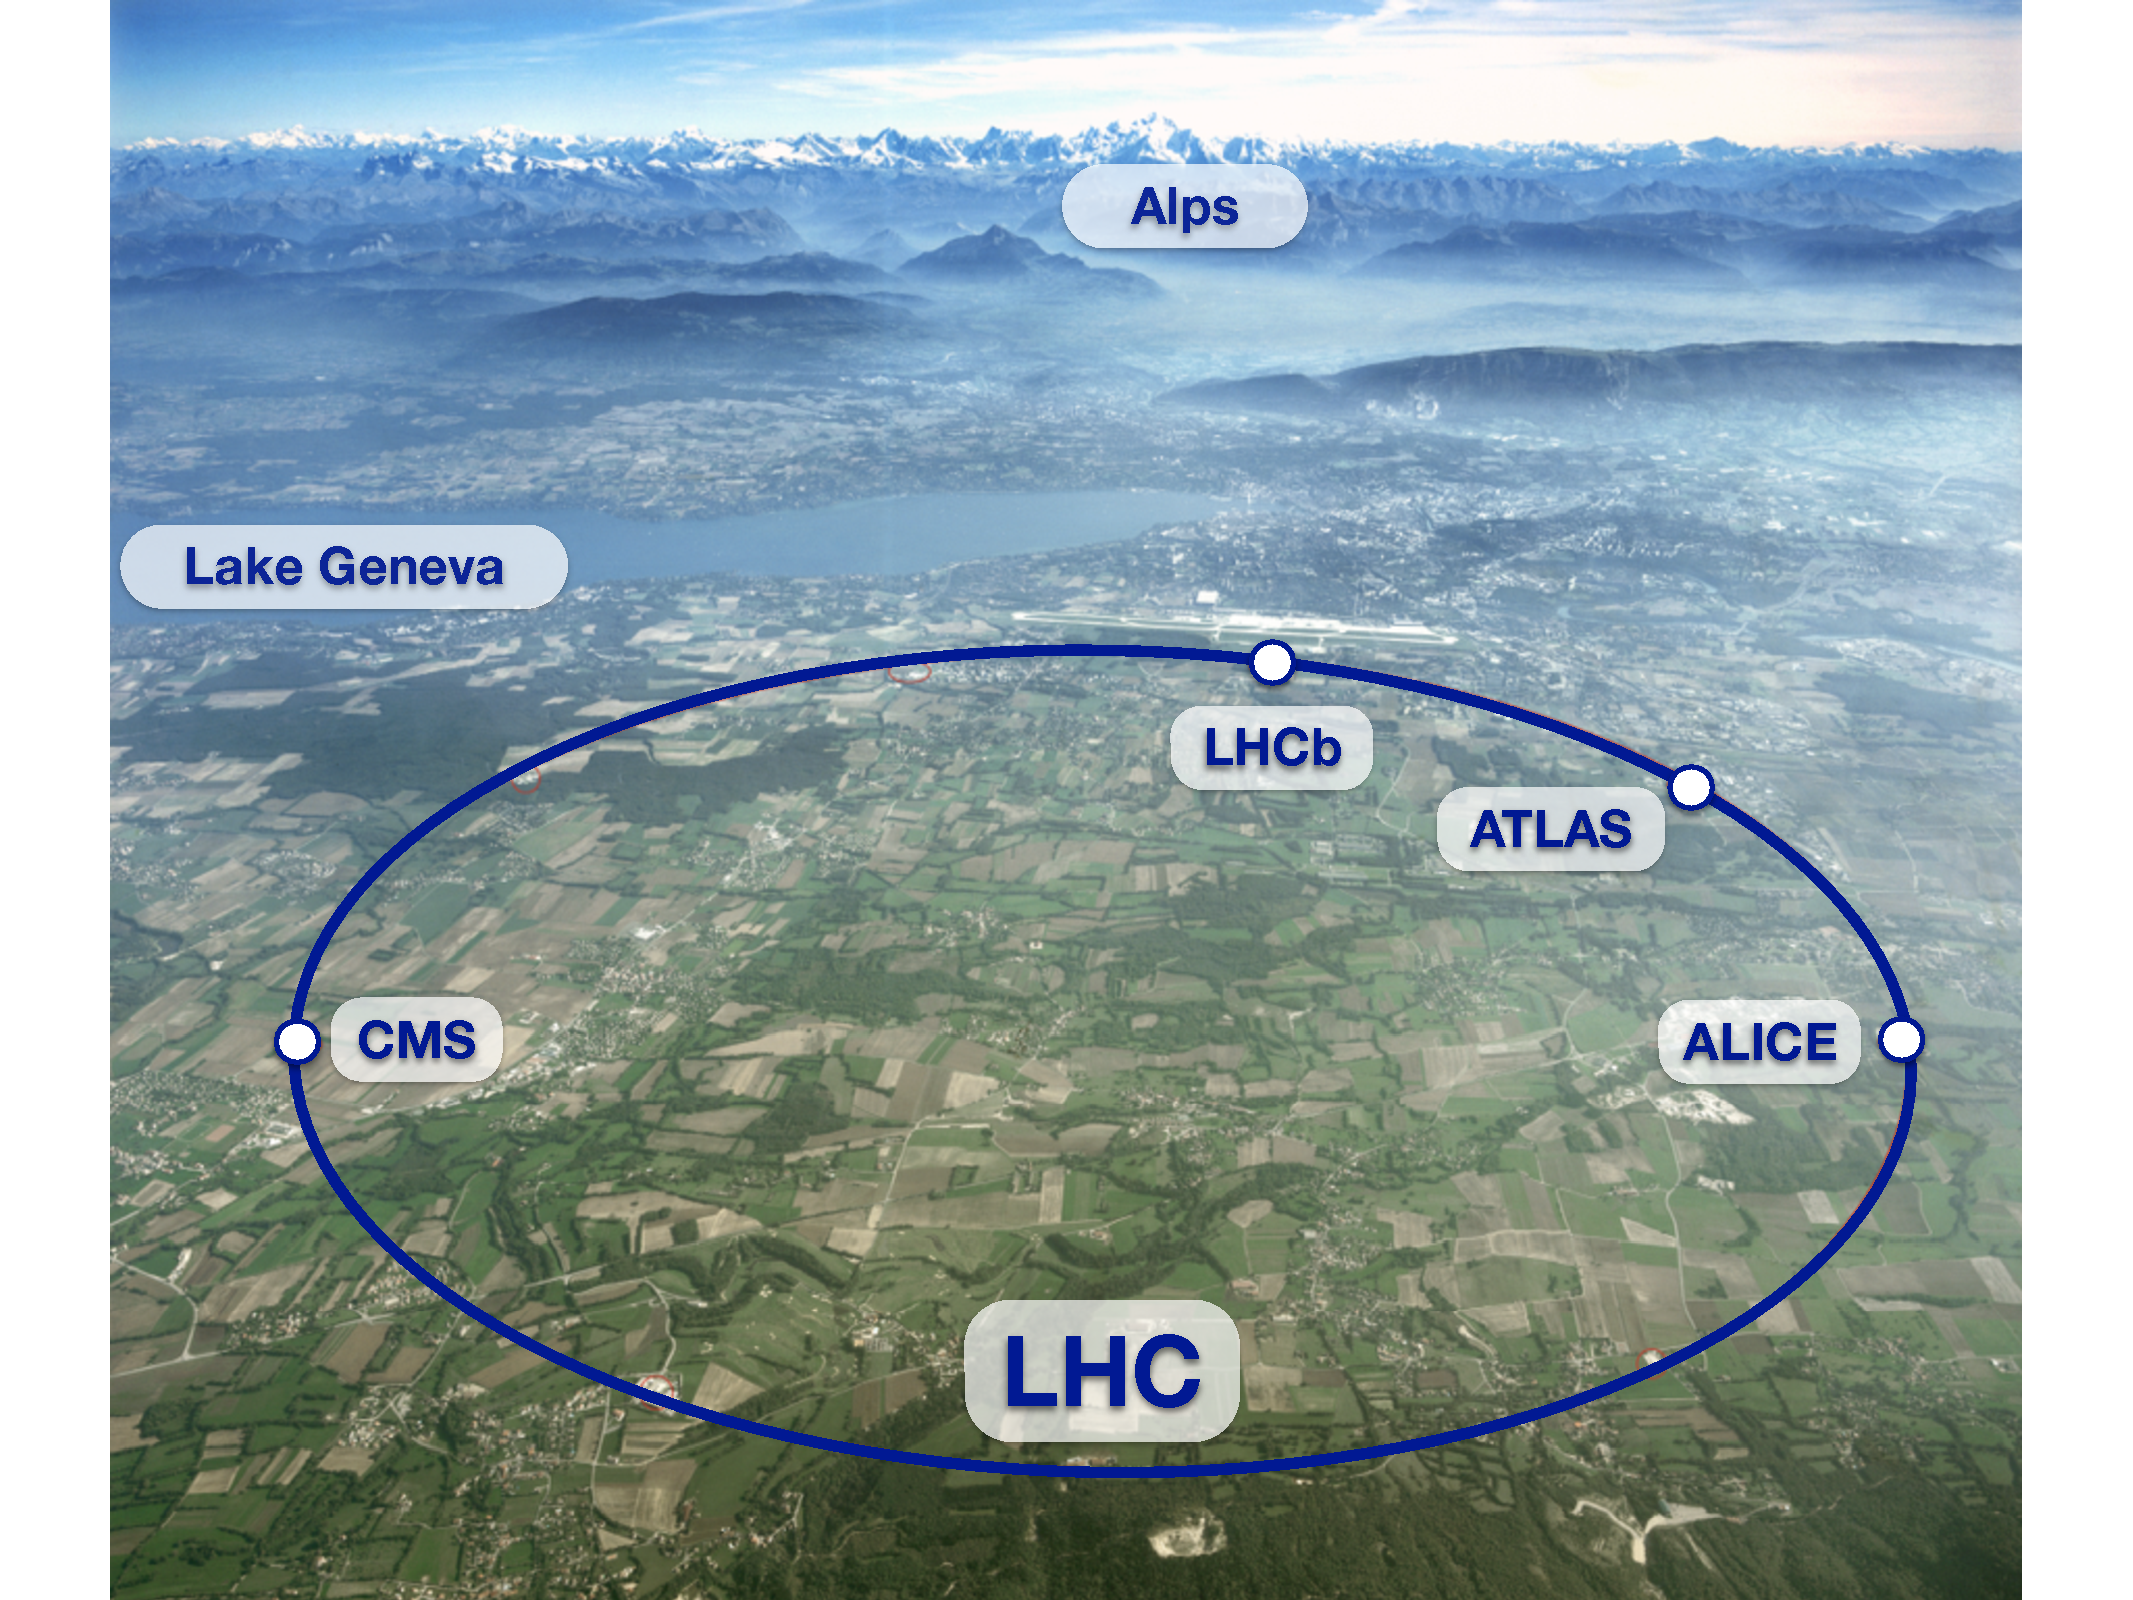
\includegraphics[width=0.75\textwidth, clip=true, trim=0 0 1cm 0]
    {figs/lhc/lhc_aerial.pdf}
  \caption{Areal view of the Geneva area with an overlaid drawing of the LHC
    and experiments~\cite{lhc_aerial}.
  }
  \label{fig:lhc_aerial}
\end{figure}

\begin{figure}[ht]
  \centering
  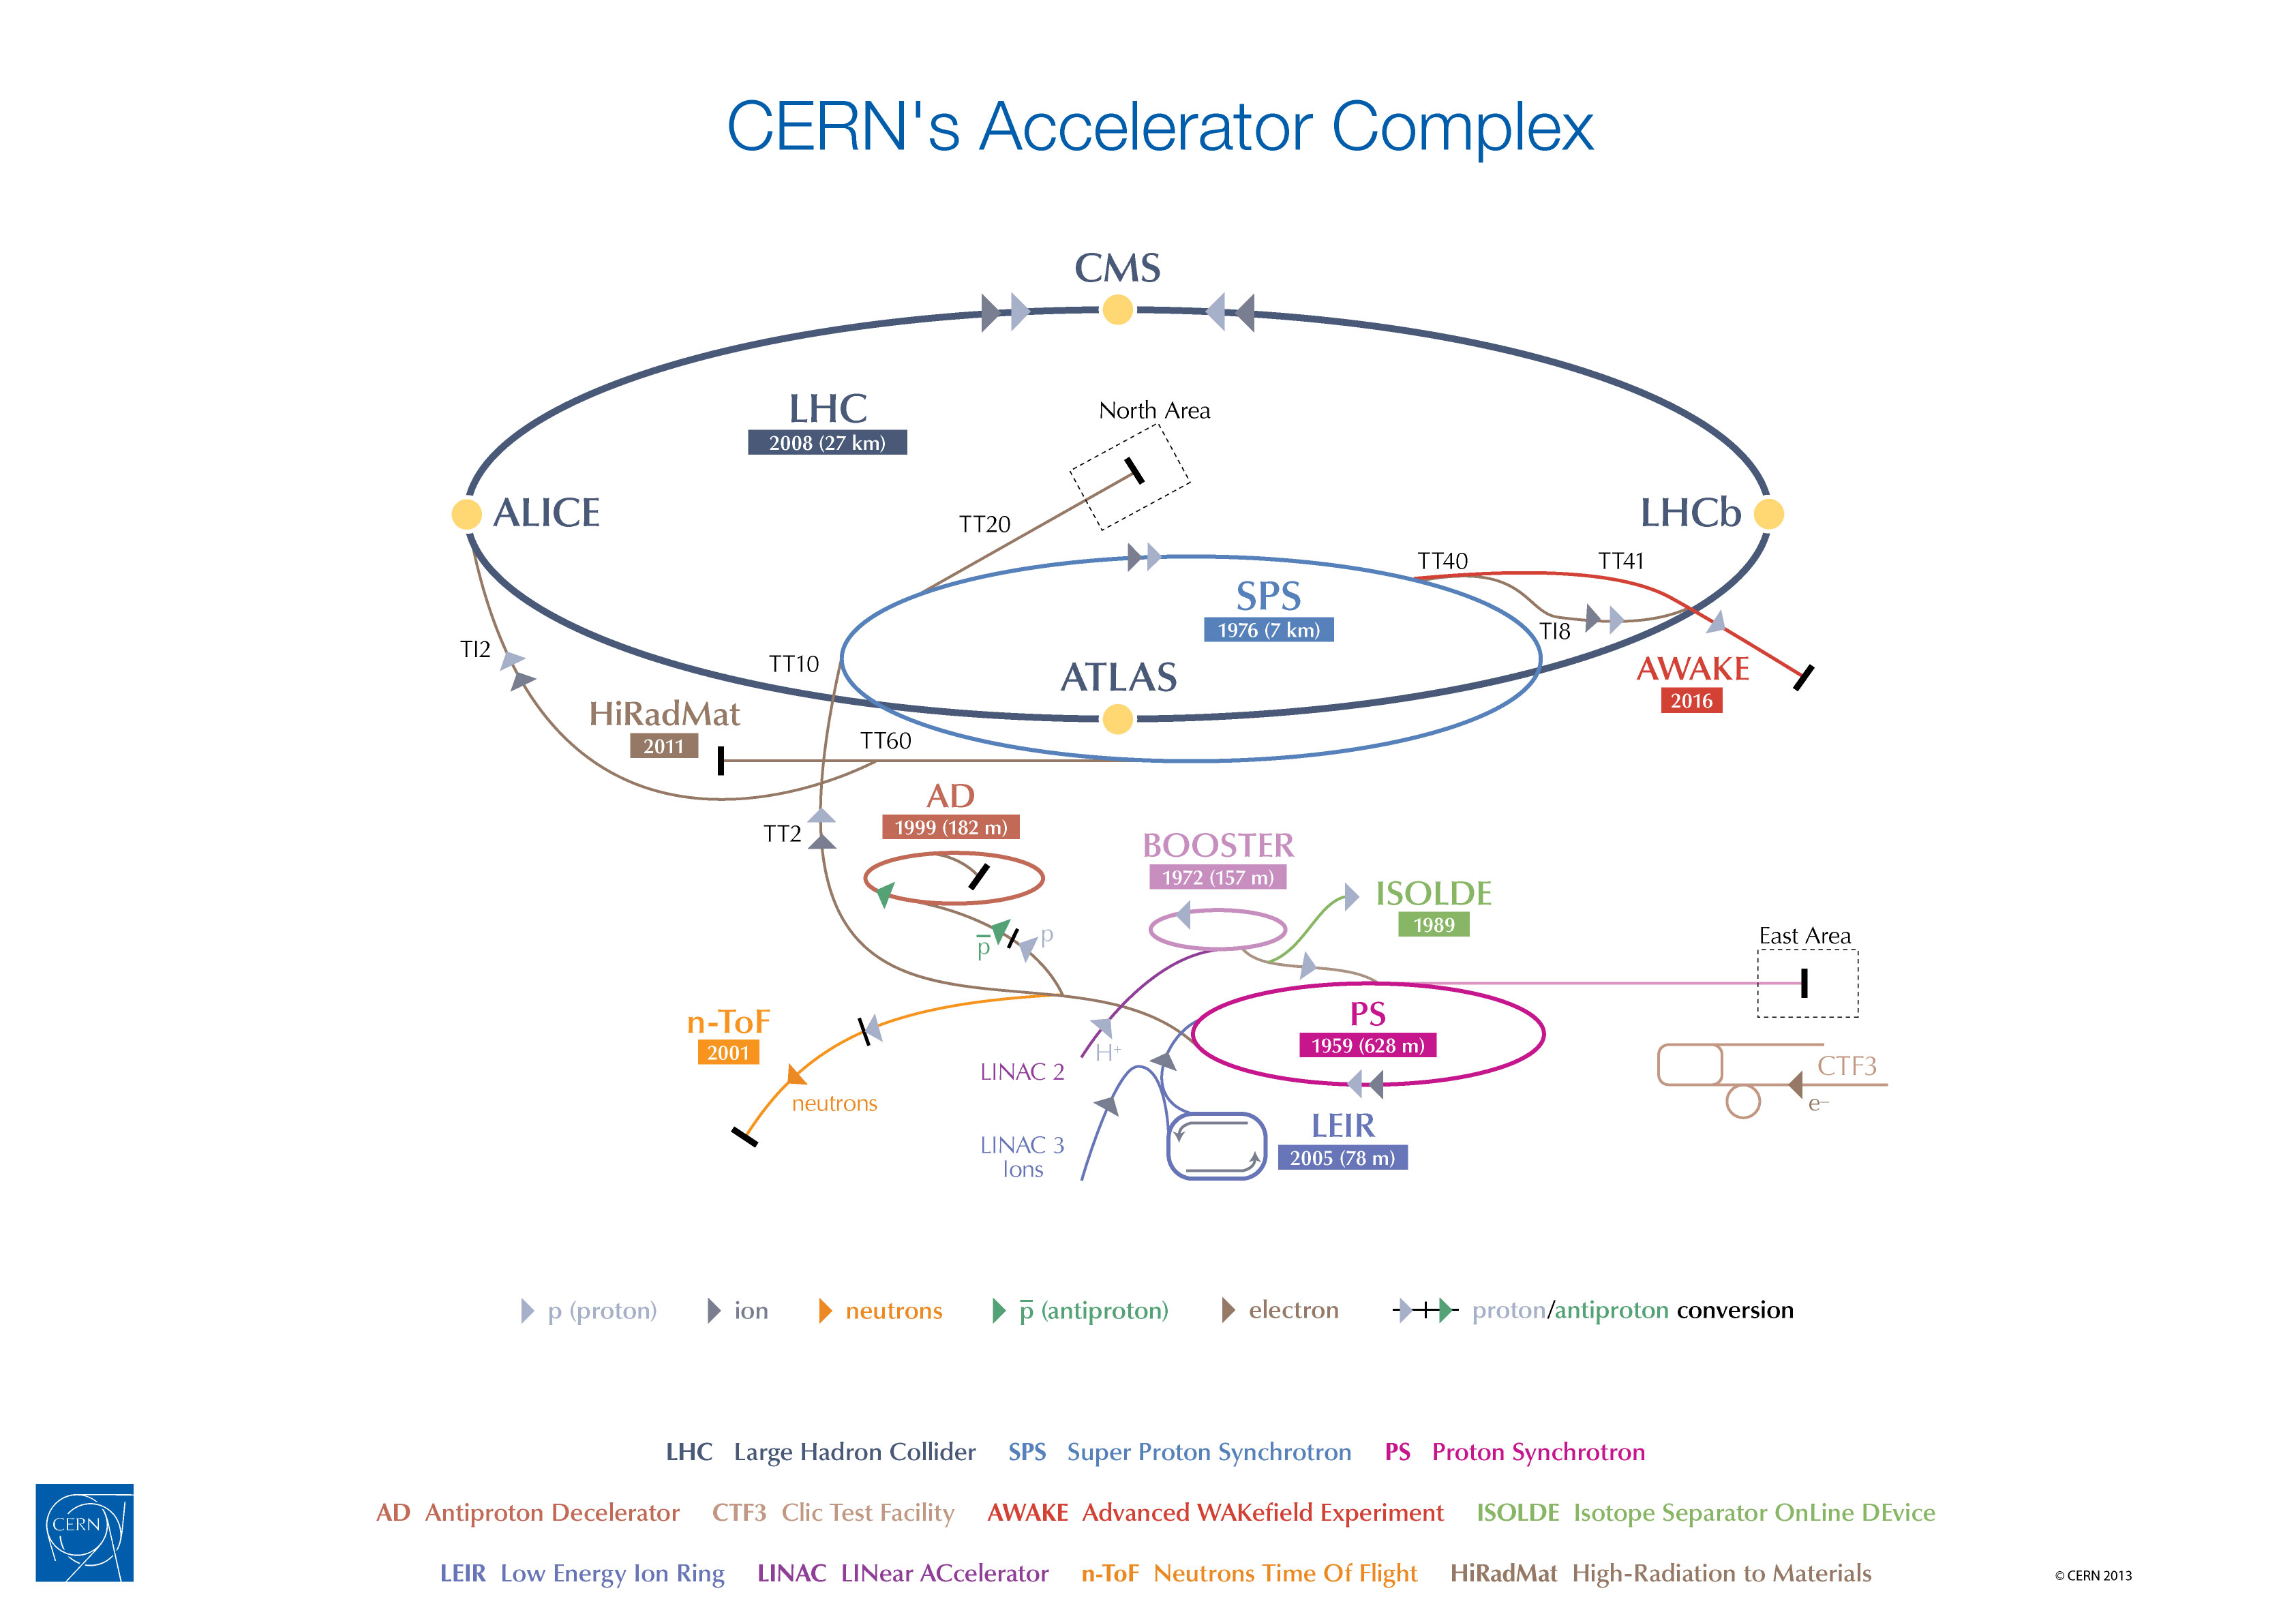
\includegraphics[width=0.75\textwidth, clip=true, trim=15cm 0 15cm 10cm]
    {figs/lhc/accelerator_complex.jpg}
  \caption{CERN accelerator complex ...~\cite{Marcastel:1621583}.
  }
  \label{fig:cern_complex}
\end{figure}

%% ------------------------------------------------------------------------------
\FloatBarrier
\section{The ATLAS experiment}

{\color{red} Brief intro to ATLAS before getting into the details}

\begin{figure}[ht]
  \centering
  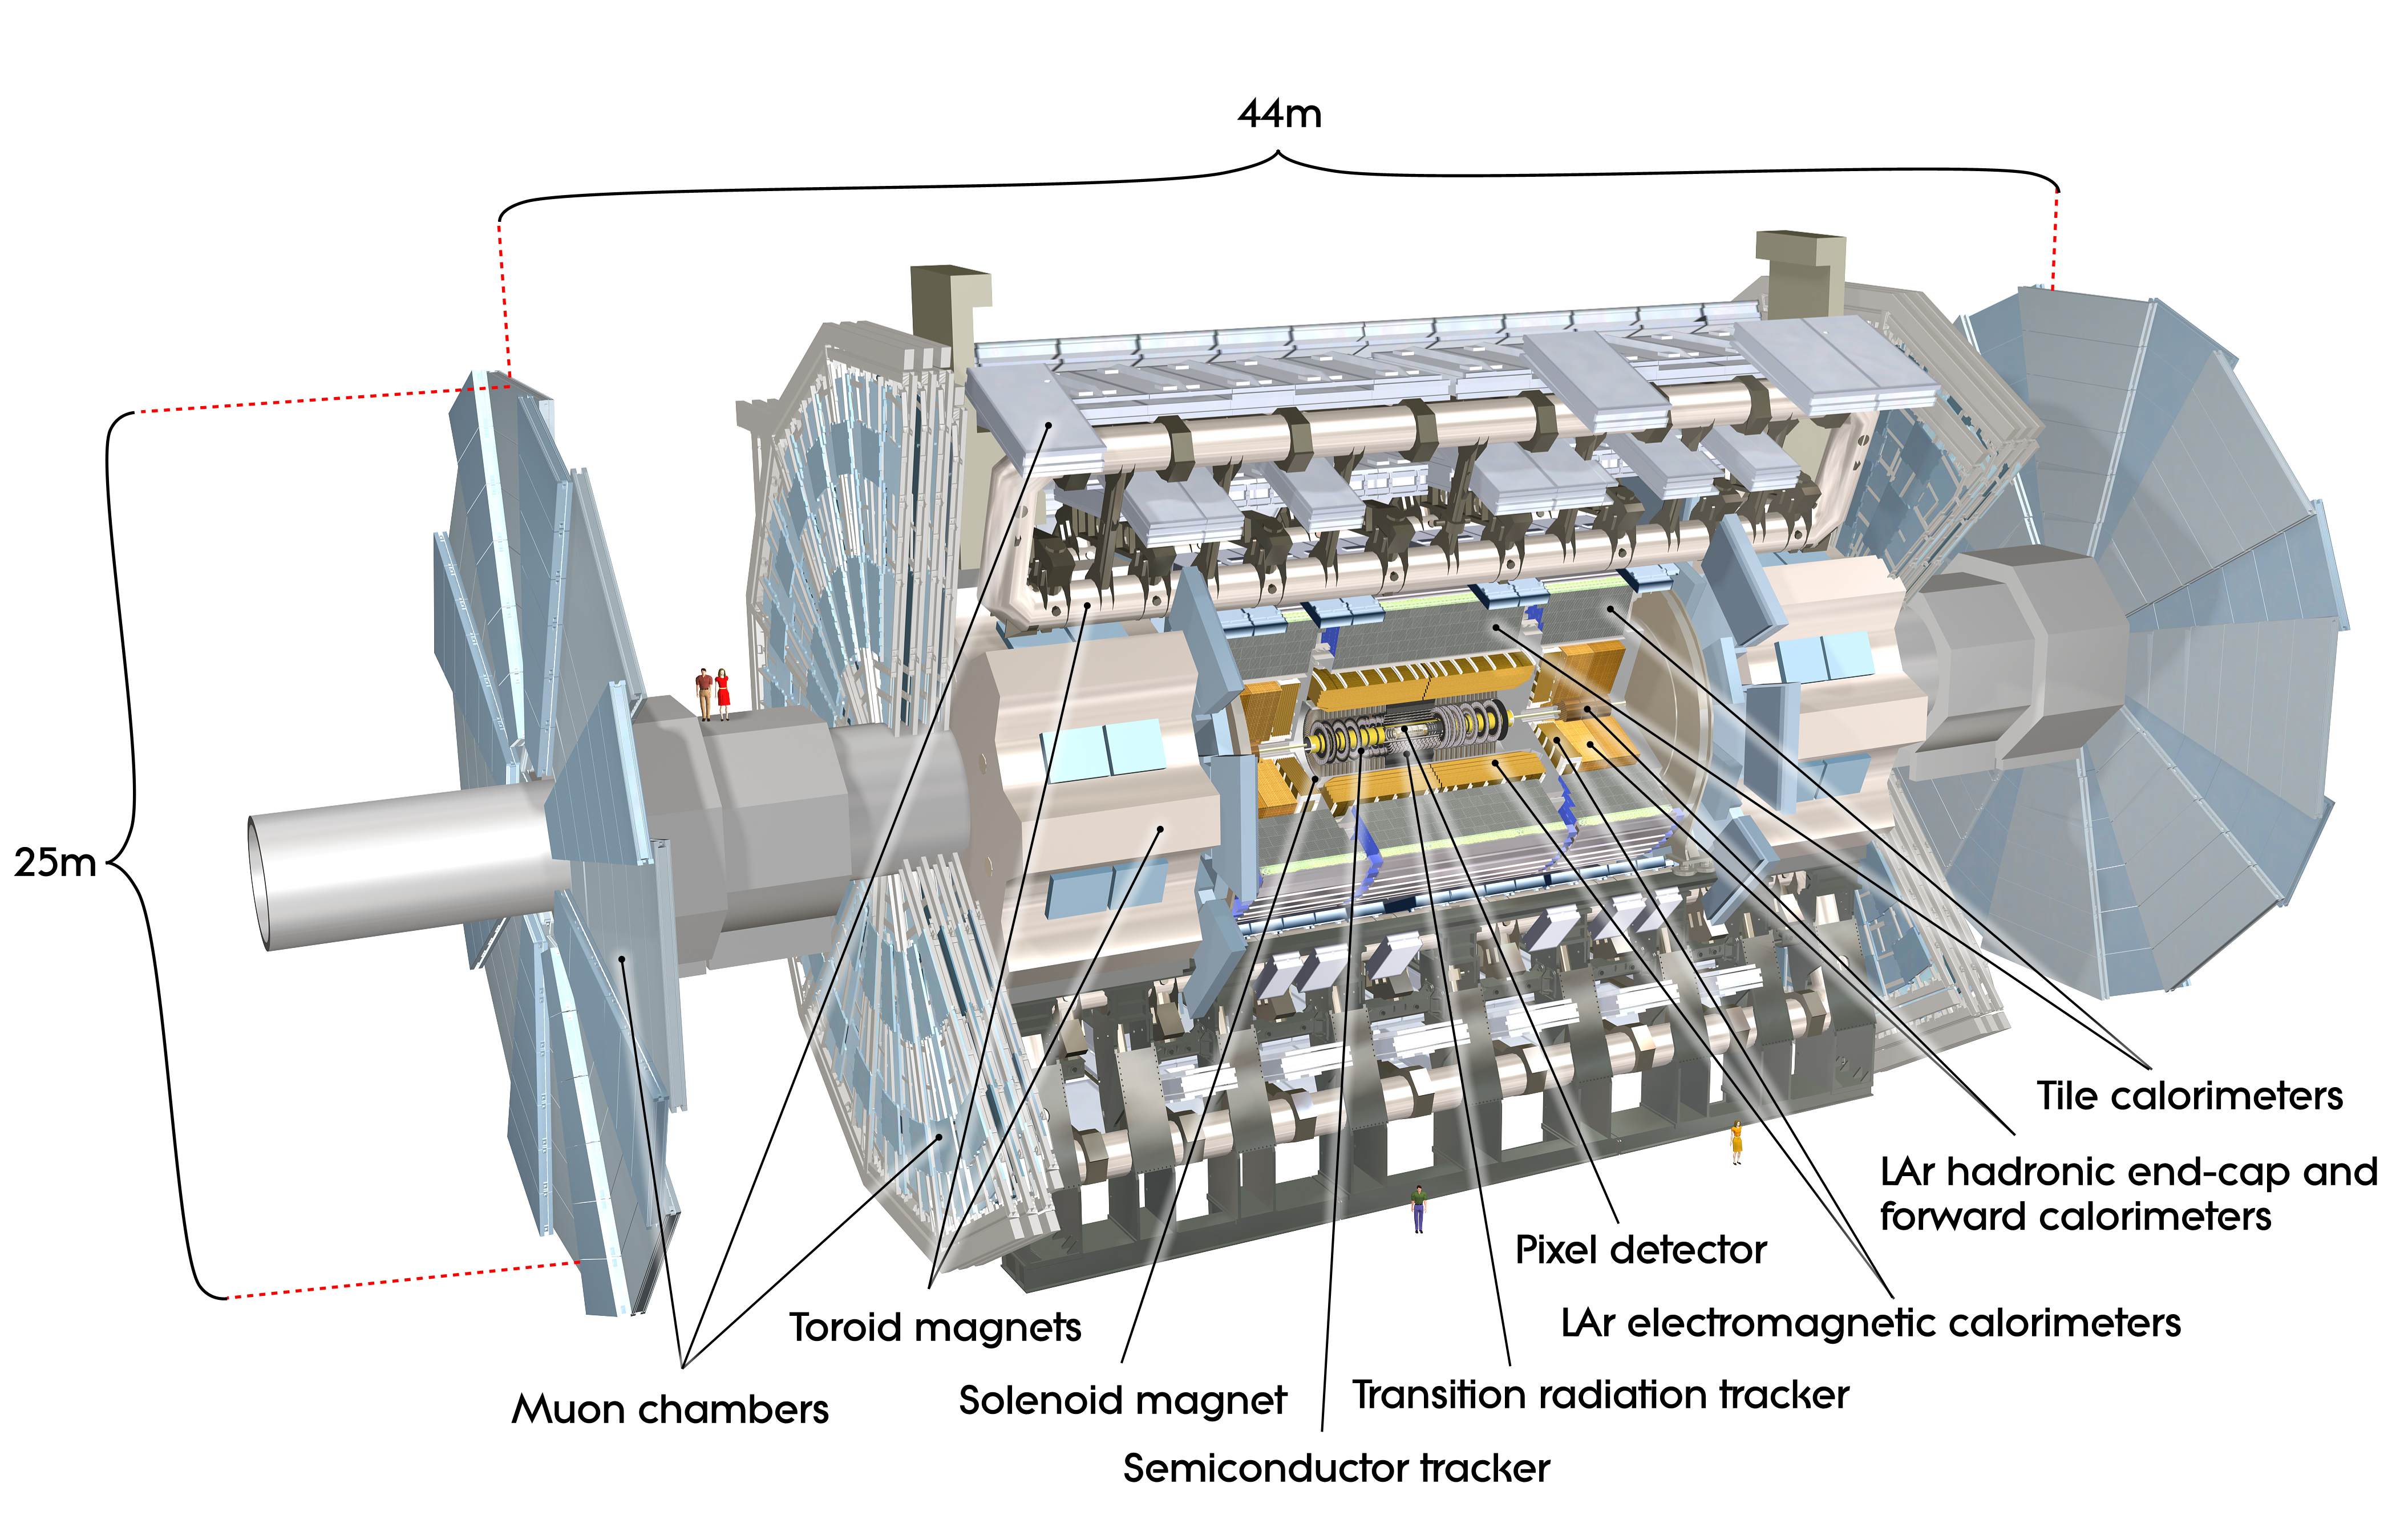
\includegraphics[width=0.75\textwidth, clip=true, trim=0 0 0 0]
    {figs/lhc/atlas_det.jpg}
  \caption{ATLAS detector ...~\cite{Pequenao:1095924}.
  }
  \label{fig:atlas_det}
\end{figure}

%% - - - - - - - - - - - - - - - - - - - - - - - - - - - - - - - - - - - - - - -
\FloatBarrier
\subsection{Inner detector} 

{\color{red} Introduce the ID and its purpose}

%% - - - - - - - - - - - - - - - - - - - - - - - - - - - - - - - - - - - - - - -
\FloatBarrier
\subsubsection{Pixel detector} 

%% - - - - - - - - - - - - - - - - - - - - - - - - - - - - - - - - - - - - - - -
\FloatBarrier
\subsubsection{Silicon semiconductor tracker} 

%% - - - - - - - - - - - - - - - - - - - - - - - - - - - - - - - - - - - - - - -
\FloatBarrier
\subsubsection{Transition radiation tracker} 

{\color{red} Brief intro to TRT. Say more is coming later in
  Chapter~\ref{ch:trt}}

{\color{red}This section should talk about how the TRT operates, going into
  what happens as a charged particle passes through the straw, and deposits
  charge, and ultimately creates a signal. Then, I can get into $rt$ curves
  and tracking performance.}

{\color{red}I know less about this than TRT tracking, but since it's one of the
  main functions of the TRT, I think it's important to at least discuss this
    briefly}

%% - - - - - - - - - - - - - - - - - - - - - - - - - - - - - - - - - - - - - - -
\FloatBarrier
\subsection{Calorimetry} 

{\color{red} Introduce the calo systems and its purpose}

%% - - - - - - - - - - - - - - - - - - - - - - - - - - - - - - - - - - - - - - -
\FloatBarrier
\subsubsection{Electromagnetic calorimeter} 

%% - - - - - - - - - - - - - - - - - - - - - - - - - - - - - - - - - - - - - - -
\FloatBarrier
\subsubsection{Hadronic calorimeter} 

%% - - - - - - - - - - - - - - - - - - - - - - - - - - - - - - - - - - - - - - -
\FloatBarrier
\subsection{Muon spectrometer} 

{\color{red} Introduce the MS and its purpose}

%% ------------------------------------------------------------------------------
\FloatBarrier
\section{Triggering system}

{\color{red} Why/how we trigger. What sort of rates we get. What is the
rejection rate at each trigger level...}

%% ------------------------------------------------------------------------------
\FloatBarrier
\section{Event reconstruction and object identification}

%% - - - - - - - - - - - - - - - - - - - - - - - - - - - - - - - - - - - - - - -
\FloatBarrier
\subsection{Electrons} 
\label{sec:elctrons}

{\color{red} TODO this is the text from the CONF note. Update and expand...}

%% - - - - - - - - - - - - - - - - - - - - - - - - - - - - - - - - - - - - - - -
\FloatBarrier
\subsection{Muons} 
\label{sec:muons}

{\color{red} TODO this is the text from the CONF note. Update and expand...}

%% - - - - - - - - - - - - - - - - - - - - - - - - - - - - - - - - - - - - - - -
\FloatBarrier
\subsection{Jets} 
\label{sec:jets}

{\color{red} TODO this is the text from the CONF note. Update and expand...}

Jets are reconstructed using the anti-$k_{t}$
algorithm~\cite{Cacciari:2008gp, Cacciari:2005hq} with a radius
parameter $R = $ 0.4 from calibrated clusters of energy deposits in
the calorimeters. The differences in calorimeter response between
electrons, photons and hadrons are taken into account by classifying
each cluster, prior to the jet reconstruction, as coming from an
electromagnetic or hadronic shower on the basis of its shape
\cite{JES}.  The jet energy thus accounts for electromagnetic
and hadronic energy deposits at the cluster level with correction
factors derived from MC simulation.  A further correction,
used to calibrate the jet energy to the scale of its constituent
particles, (JES) \cite{JES,JES2}, is then applied.  The impact of
pileup is accounted for using
a technique, based on jet areas, that provides an event-by-event and
jet-by-jet correction \cite{Cacciari:2007fd}.  Jets are required
to have transverse momentum \pt\ $>$ 40~\GeV\ and $|\eta| < 4.9$.
In order to reduce contamination from jets produced by pileup,
the scalar sum of the \pt of the tracks matched to the jet and
originating from the primary vertex must be at least 50\% of the
scalar sum of the \pt of all tracks matched to the jet.  This
criterion is only applied to jets with \pt $<$ 50~\GeV\ and $|\eta| < 2.4$.

%% - - - - - - - - - - - - - - - - - - - - - - - - - - - - - - - - - - - - - - -
\FloatBarrier
\subsection{Flavor tagging} 
\label{sec:flavor_tagging}

{\color{red} TODO this is the text from the CONF note. Update and expand...}

The identification of $b$-jets uses the MV1 flavor tagging
algorithm~\cite{ATLAS-CONF-2014-004, ATLAS-CONF-2014-046}, which is
based on an artificial neural network
algorithm that exploits the impact parameters of charged particle
tracks, the parameters of reconstructed secondary vertices, and the
topology of $b$- and $c$-hadron decays inside a jet.  The operating
point corresponds to an overall 80\% $b$-tagging efficiency, as
measured in simulated \TTBAR\ events, to a rejection factor of 25 for jets
originating from light quarks or gluons, and to a rejection factor of
3 for jets originating from charm quarks.

%% - - - - - - - - - - - - - - - - - - - - - - - - - - - - - - - - - - - - - - -
\FloatBarrier
\subsection{Missing energy} 
\label{sec:met}

{\color{red} missing momentum?}
{\color{red} TODO this is the text from the CONF note. Update and expand...}

The vector momentum imbalance in the transverse plane is obtained from
the negative vector sum of the reconstructed and calibrated physics
objects and the calorimeter energy clusters not associated with reconstructed
objects. This is denoted as missing transverse momentum, and the symbol
$\met$ is used for its magnitude.  The $\met$ calculation is described
elsewhere~\cite{ATLAS-CONF-2013-082}.
